\documentclass[conference]{IEEEtran}

\usepackage[spanish]{babel}
\usepackage[utf8]{inputenc}
\usepackage{cite}
\usepackage{amsmath, amsthm,amssymb,amsfonts}
\usepackage{algorithmic}
\usepackage{graphicx}
\usepackage{textcomp}
\usepackage{xcolor}
\def\BibTeX{{\rm B\kern-.05em{\sc i\kern-.025em b}\kern-.08em
    T\kern-.1667em\lower.7ex\hbox{E}\kern-.125emX}}

% Definición del entorno 'definition'
\newtheorem{definition}{Definición}

\begin{document}
\title{Consenso en Sistemas Euler-Lagrange con Retardos y Perturbaciones Desconocidas	% {\footnotesize \textsuperscript{*}Note: Sub-titles are not captured in Xplore and
	% should not be used}
	% \thanks{Identify applicable funding agency here. If none, delete this.}
}

\author{
	\IEEEauthorblockN{José Alejandro León Sánchez}
	\IEEEauthorblockA{\textit{Posgrado de Ingeniería} \\
		\textit{UNAM}\\
		CDMX, Mexico}
	\and
	\IEEEauthorblockN{Emmanuel Nuño Ortega}
	\IEEEauthorblockA{\textit{Universidad de Guadalajara} \\
		% \textit{}\\
		Jalisco, Mexico}
}

\maketitle

\begin{abstract}
    Este trabajo analiza el problema de consenso en redes de sistemas multi-agente descritos por dinámicas Euler-Lagrange. Se presentan retos significativos, como retardos en la comunicación entre nodos y la presencia de perturbaciones externas desconocidas. Para abordar estas dificultades, se propone un esquema de control adaptativo con inyección de amortiguamiento y estimación de perturbaciones mediante modelos internos. Los resultados teóricos y simulaciones confirman la estabilidad del sistema y la convergencia exponencial hacia el consenso, incluso bajo condiciones dinámicas adversas.
\end{abstract}

\begin{IEEEkeywords}
    Consenso, sistemas Euler-Lagrange, control distribuido, retardos, estimación de perturbaciones.
\end{IEEEkeywords}

\section*{Introducción}

El consenso en sistemas multi-agente es un área clave en robótica distribuida y sistemas dinámicos. El objetivo principal es garantizar que todos los agentes de una red, ya sean robots, drones o sistemas mecánicos, alcancen un acuerdo sobre un estado común, como una posición o trayectoria deseada. Este desafío se magnifica cuando los agentes poseen dinámicas complejas, como las descritas por los sistemas Euler-Lagrange, donde la presencia de retardos en la comunicación y perturbaciones desconocidas pueden desestabilizar el sistema.

Durante la ponencia se destacó el uso de técnicas avanzadas de control adaptativo, junto con modelos internos para estimación dinámica, como una solución robusta frente a estas limitaciones. Este enfoque se basa en el diseño de esquemas que no requieren el conocimiento previo de las frecuencias de las perturbaciones, ofreciendo una solución escalable y eficiente para aplicaciones reales.

\section*{Modelado de Sistemas Euler-Lagrange}

Los sistemas Euler-Lagrange (EL) representan una clase de sistemas dinámicos ampliamente utilizada en robótica y mecánica. Su comportamiento se describe mediante las ecuaciones:
\[
M_i(q_i)\ddot{q}_i + C_i(q_i, \dot{q}_i)\dot{q}_i + \frac{\partial}{\partial q_i} U(q_i) = \tau_i + \delta_i(t),
\]
donde:
\begin{itemize}
    \item \( q_i \): posición generalizada del agente \( i \).
    \item \( M_i \): matriz de inercia, dependiente de la configuración.
    \item \( C_i \): matriz de Coriolis, que captura los efectos de velocidad relativa.
    \item \( U(q_i) \): energía potencial del sistema.
    \item \( \tau_i \): entrada de control aplicada al sistema.
    \item \( \delta_i(t) \): perturbaciones externas no modeladas.
\end{itemize}

El problema de consenso se define en términos de convergencia a una posición o trayectoria común, considerando dos escenarios: uno sin líder, donde todos los agentes se sincronizan entre sí, y otro con líder, donde un agente principal guía el comportamiento de la red.

\begin{figure}[h!]
    \centering
    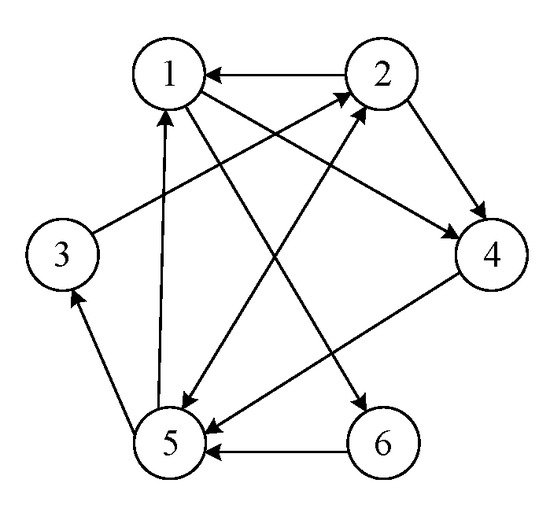
\includegraphics[width=0.5\textwidth]{network.jpg}
    \caption{Representación de una red de sistemas Euler-Lagrange}
\end{figure}

\section*{Esquema de Control Propuesto}

Para mitigar los efectos de retardos y perturbaciones, se propone un controlador basado en inyección de amortiguamiento, descrito matemáticamente por:
\[
\tau_i = -\hat{\delta}_i - p_i \sum_{j \in N_i} a_{ij} (q_i - q_j(t - T_{ij}(t))) - d_i\dot{q}_i + \frac{\partial}{\partial q_i} U(q_i),
\]
donde:
\begin{itemize}
    \item \( p_i \): ganancias que determinan la velocidad de convergencia.
    \item \( \hat{\delta}_i \): estimación de perturbaciones externas.
    \item \( T_{ij}(t) \): retardo variable entre agentes \( i \) y \( j \).
\end{itemize}

El controlador utiliza técnicas de observación para estimar las perturbaciones y garantiza que las diferencias entre perturbación real (\( \delta_i \)) y estimada (\( \hat{\delta}_i \)) converjan a cero exponencialmente. Este enfoque es particularmente efectivo en sistemas con retardos temporales, al permitir ajustes dinámicos y robustos en tiempo real.



\section*{Estimación de Perturbaciones}

Las perturbaciones externas se modelan como combinaciones de señales sinusoidales de frecuencias desconocidas. El esquema de estimación se basa en la implementación de observadores dinámicos y algoritmos de mínimos cuadrados extendidos. Esto permite calcular parámetros clave y lograr convergencia exponencial, asegurando que las acciones de control sean precisas incluso en presencia de perturbaciones no previstas.

\section*{Conclusiones}

El esquema de control propuesto combina estrategias adaptativas con estimación de perturbaciones para abordar retos complejos en redes de sistemas Euler-Lagrange. Se garantiza la estabilidad del sistema, incluso bajo condiciones adversas como retardos temporales y perturbaciones desconocidas. Los resultados obtenidos abren la puerta a futuras investigaciones en redes multi-agente con topologías dinámicas, así como en aplicaciones experimentales con robots colaborativos.

\end{document}